\chapter{The CMS Experiment and the CERN LHC}

\section{The LHC}

\subsection{LHC Pre-Acceleration}

\subsection{LHC Acceleration}

\section{The CMS Experiment}

The Compact Muon Solenoid (CMS) detector is located at point 5 along the LHC ring near Cessy, France. It is
one of the two large general purpose physics detectors in operation at the LHC along with ATLAS. The
CMS detector was inspired by decades of previous high energy particle physics detectors and has as its
primary purpose to detect and measure the characteristics of the Standard Model Higgs boson. The 
detector was designed and built targeting high efficiency and energy resolution for specific Higgs 
boson decay modes. The high granularity of the electromagnetic calorimeter and excellent energy
resolution make it perfect for reconstructing photons from $\PH \to \gamma\gamma$ decays. The
strong, 3.8T magnetic field combined with the muon spectrometer provide excellent Higgs boson
mass resolution in the $\PH \to \PZ\PZ \to \Pgm\Pgm\Pgm\Pgm$ decays. The detector is a large
cylinder 15.0m in diameter and 28.7m in length. It has a mass of approximately 14,000,000kg.

The CMS detector is built out of many subdetectors. Progressing radially outwards from the collision point,
there is firts the silicon pixel tracker the the silicon strip trigger sytems. Next is the 
electromagnetic calorimeter followed by the hadronic calorimeter. These systems are all contained
within the bore of the CMS superconducting magnet. After the the solenoid there are additional subsystems
embedded within the steel flux-return yoke. In the central region of the detector, there is an 
outer portion of the hadronic calorimeter, and lastly, the muon spectrometer. These systems can all be viewd in
Figure~\ref{fig:cms_detector}.

\begin{figure*}[htbp]
\centering
     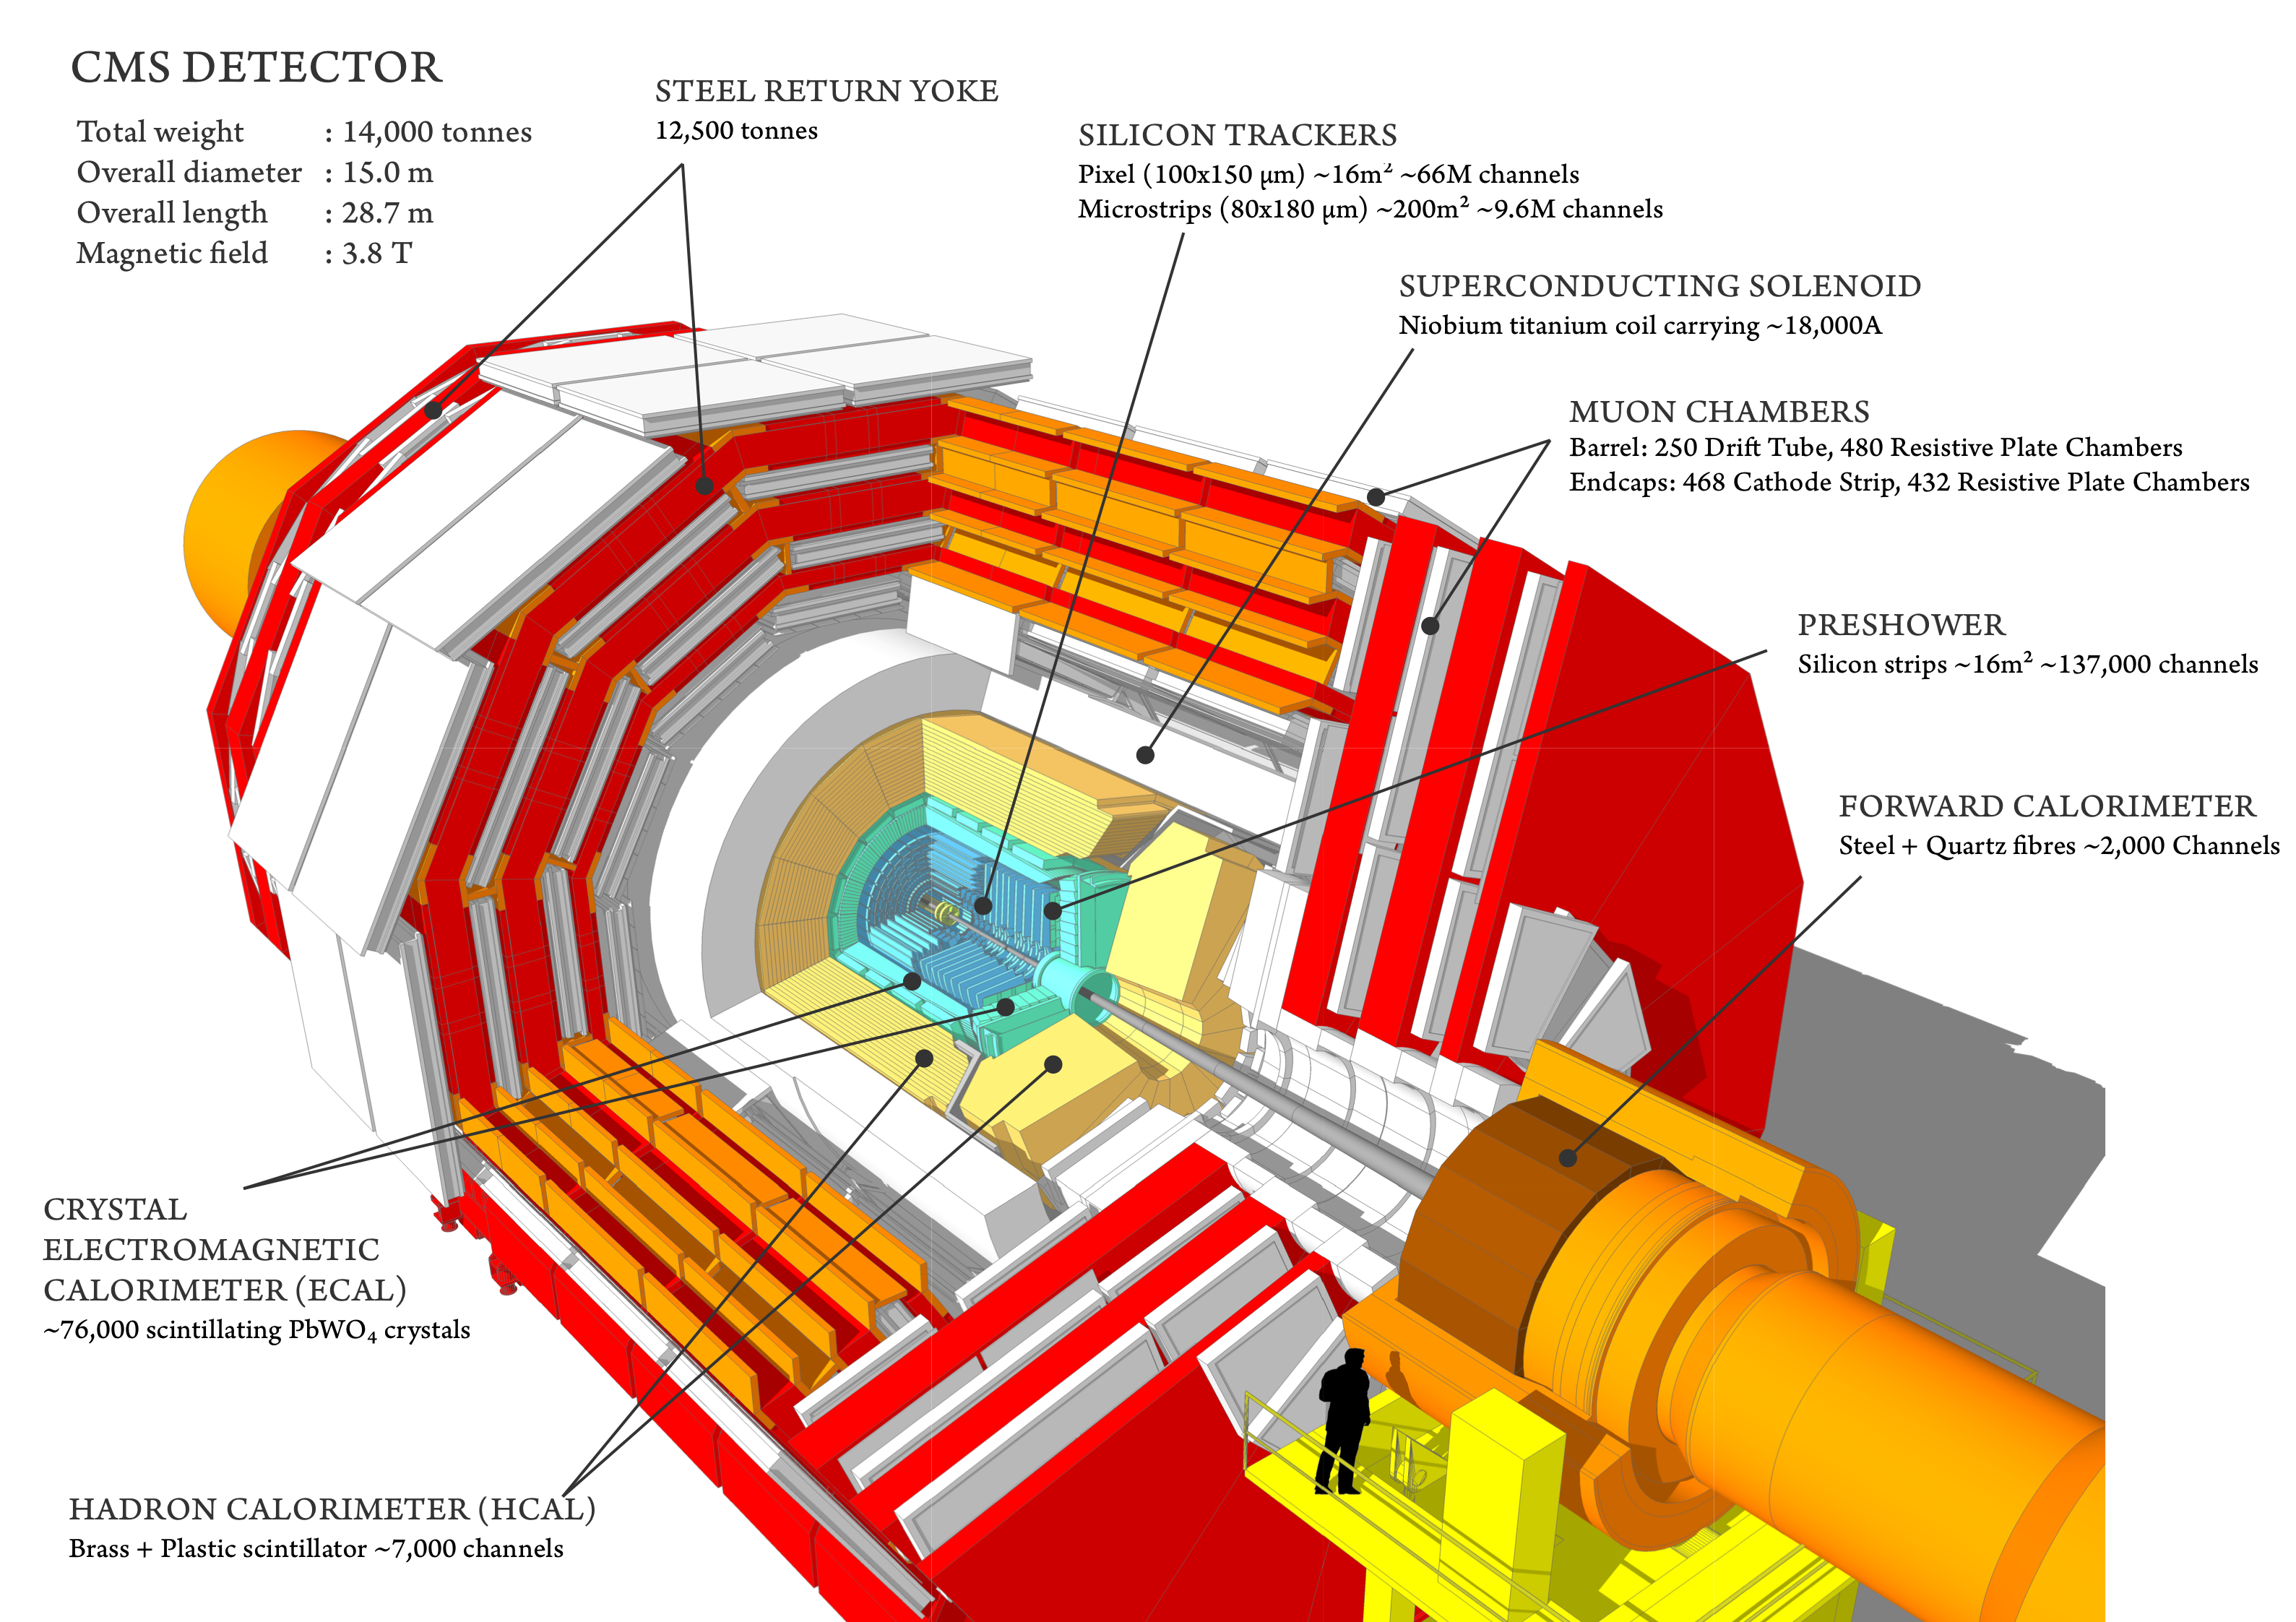
\includegraphics[width=1.0\textwidth]{cms_and_lhc/plots/cms_detector.png}
     \caption{
     }
     \label{fig:cms_detector}
\end{figure*}

Information from the 40 MHz proton-proton collisions is aggregated by a central data acquisition system
and filtered before storage by a two-tiered trigger system~\cite{Khachatryan:2016bia}. 
The first level of the trigger sytem is composed of custom hardware processors, uses information 
from the calorimeters and muon detectors to select events at a rate of around 100 kHz. The second level of
the trigger, known as the high-level trigger, consists of a farm of commercial processors further
filtering out non-interesting data events resulting in a final event rate of about 1 kHz which is stored
for futher processing an analysis.



\subsection{Geometry}
To understand the CMS detector, an understanding of the geometry and coordinate system used by the 
CMS detector is necessary. The CMS detector is a hermetic, cylindrical particle detector surrounding
a central region designed to be the location of the $\pp$ collisions delivered LHC. This middle
point, inside the LHC beam pipe is designated as the origin for the CMS coordinate system, (0,0,0) in
$(x, y, z)$ coordinates. Positive $x$ points towards the center of the LHC ring.
Positive $y$ points vertically upwards. The positive $z$ direction is along the LHC ring in the
clockwise direction when viewed from above. These $(x, y, z)$ coordinates are commonly transformed
into quasicylindrical coordinates when referring to particles, $(\pt, \eta, \phi)$. For a particle,
$\pt$ is:

\begin{equation}
\pt \equiv \sqrt{p^{2}_{x} + p^{2}_{y}}
\end{equation}

$\eta$ is defined using $\theta$ from traditionally spherical coordinates.

\begin{equation}
\eta \equiv -ln\bigg[\tan\bigg(\frac{\theta}{2}\bigg)\bigg]
\end{equation}

$\phi$ is defined in the $x-y$ plane.



\subsection{Superconducting Magnet}
The CMS superconducting magnet, as is noted in the collaboration name, is one of the most fundamental
pieces of the CMS experiment. The superconducting magnet bends the trajectories of charged particles
within the CMS detector. The curve in the flight path of a charged particle can be used to help
calculate the energy or momentum of the particle in accordance with the Lorenetz force.
Within the CMS detector, where the electric field is negligible compared to the magnetic field
from the superconducting magnet, the Lorentz force can be written as~\ref{eqn:lorentz}

\begin{equation}
\textbf{F} = q\textbf{v} \times \textbf{B}
\label{eqn:lorentz}
\end{equation}

relating the mass, acceleration and momentum of a particle with the magnetic field.

The CMS superconducting magnetic is constructed from a 4-layer winding of stabalised
reinfored NbTi conductor. When in operation, the magnet is kept in a superconducting state
by cooling it with liquid helium to a temperature of 4.6 Kelvin. With a nominal current
of 19.14 kA the superconducting solenoid magnet is able to produce a roughly uniform
magnetic field of 3.8 T within its central bore. The magnetic field created is roughly
100,000 times stronger than the Earth's magnetic field. Stronger the magnetic fields produce
more higly curved particle trajectories leading to better momentume and energy measurements.
The central bore is only 6.3 m in diameter
leaving limited room for the CMS tracker and calorimeter systems.



\subsection{Inner Tracking System}
The inner tracking system is composted of two subdetectors, the pixel tracker and the
strips tracker. They are designed to deliver precise and efficient measurement of
the trajectories of charged particles propagating outwards from the LHC delivered
$\pp$ collisions. The tracking systems can be used to reconstruct the origins of
the tracks to reconstruct collision points and secondary decay vertices. The
tracking systems surround the interaction point and have a length of 5.8m and 
diameter of 2.5m. Both the pixel and strip trackers have cylindrical barrel
layers and disk-like endcap layers. A schematic of the track systems
can be seen in Figure~\ref{fig:cms_tracker}.

The pixel tracker has three barrel layers at radii between 4.4cm and 10.2cm. The
close proximity to the interaction point is helpful for track seeding and vertex
reconstruction discussed in the track reconstruction section~\ref{sec:pf_tracks}.
The silicon strip tracker is composed of 10 barrel detection layers extending 
outwards to a radius of 1.1m. During the 2016-2017 extended year end techincal stop,
the pixel tracker was upgraded to have a fourth detection layer. As 2017 data is not used
in the analyses presented here, details of this upgrade are omitted.
The endcaps of the pixel tracker consist of 2 disks which extend the $\eta$ 
range of the detector to $\abs\eta < 2.5$. The same $\eta$ range is covered in the
strips tracker with 12 disks on each side of the barrel.

\begin{figure*}[htbp]
\centering
     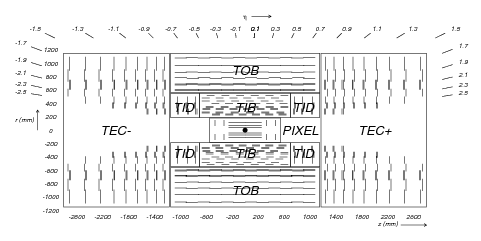
\includegraphics[width=0.8\textwidth]{cms_and_lhc/plots/cms_tracker.png}
     \caption{
Schematic cross section through the CMS tracker. Each line represents a detector module. 
Double lines indicate back-to-back modules which deliver stereo hits.
     }
     \label{fig:cms_tracker}
\end{figure*}

The pixel tracker contains about 66 million individual pixels. The strips tracker
contains 9.3 million individual strips. This phenominal resolution is necessary
because of the extremely high particle flux through the tracker. During 2016 data
taking, it is estimated that there were $\mathcal{O}( 1000 )$ particles 
traversing the tracker from the more than 20 overlapping simultaneous proton-proton 
interactions during a single bunch crossing. The tracker measures the $\pt$ of 
charged hadrons in the barrel region with a resolution of 1\% for $\pt < 20\GeV$.
The information from the tracker systems is
not used by the L1 trigger. However, the tracker information is heavily used by the HLT to
reduce the event rate from the L1 trigger, 100kHz, to the final rate of 100Hz.

A serious concern during the design of the tracker systems was the amount of
material necessary to build the systems. All of the electronics, hardware, 
cooling systems and wiring contribute to the tracker material budget. Any and all material
located between the interaction region and the calorimeters will reduce the precision 
of the calorimeter energy measurements as well as potentially degrade the track-based
measurement of the energy of a particle. This is because of potential electromagnetic
and/or nuclear interactions between the particle and the tracker material. Figure~\ref{fig:cms_tracker_thickness}
shows the material budget in terms of interaction lengths and radiation lengths as a function
of $\eta$ for the tracker systems.

\begin{figure*}[htbp]
\centering
     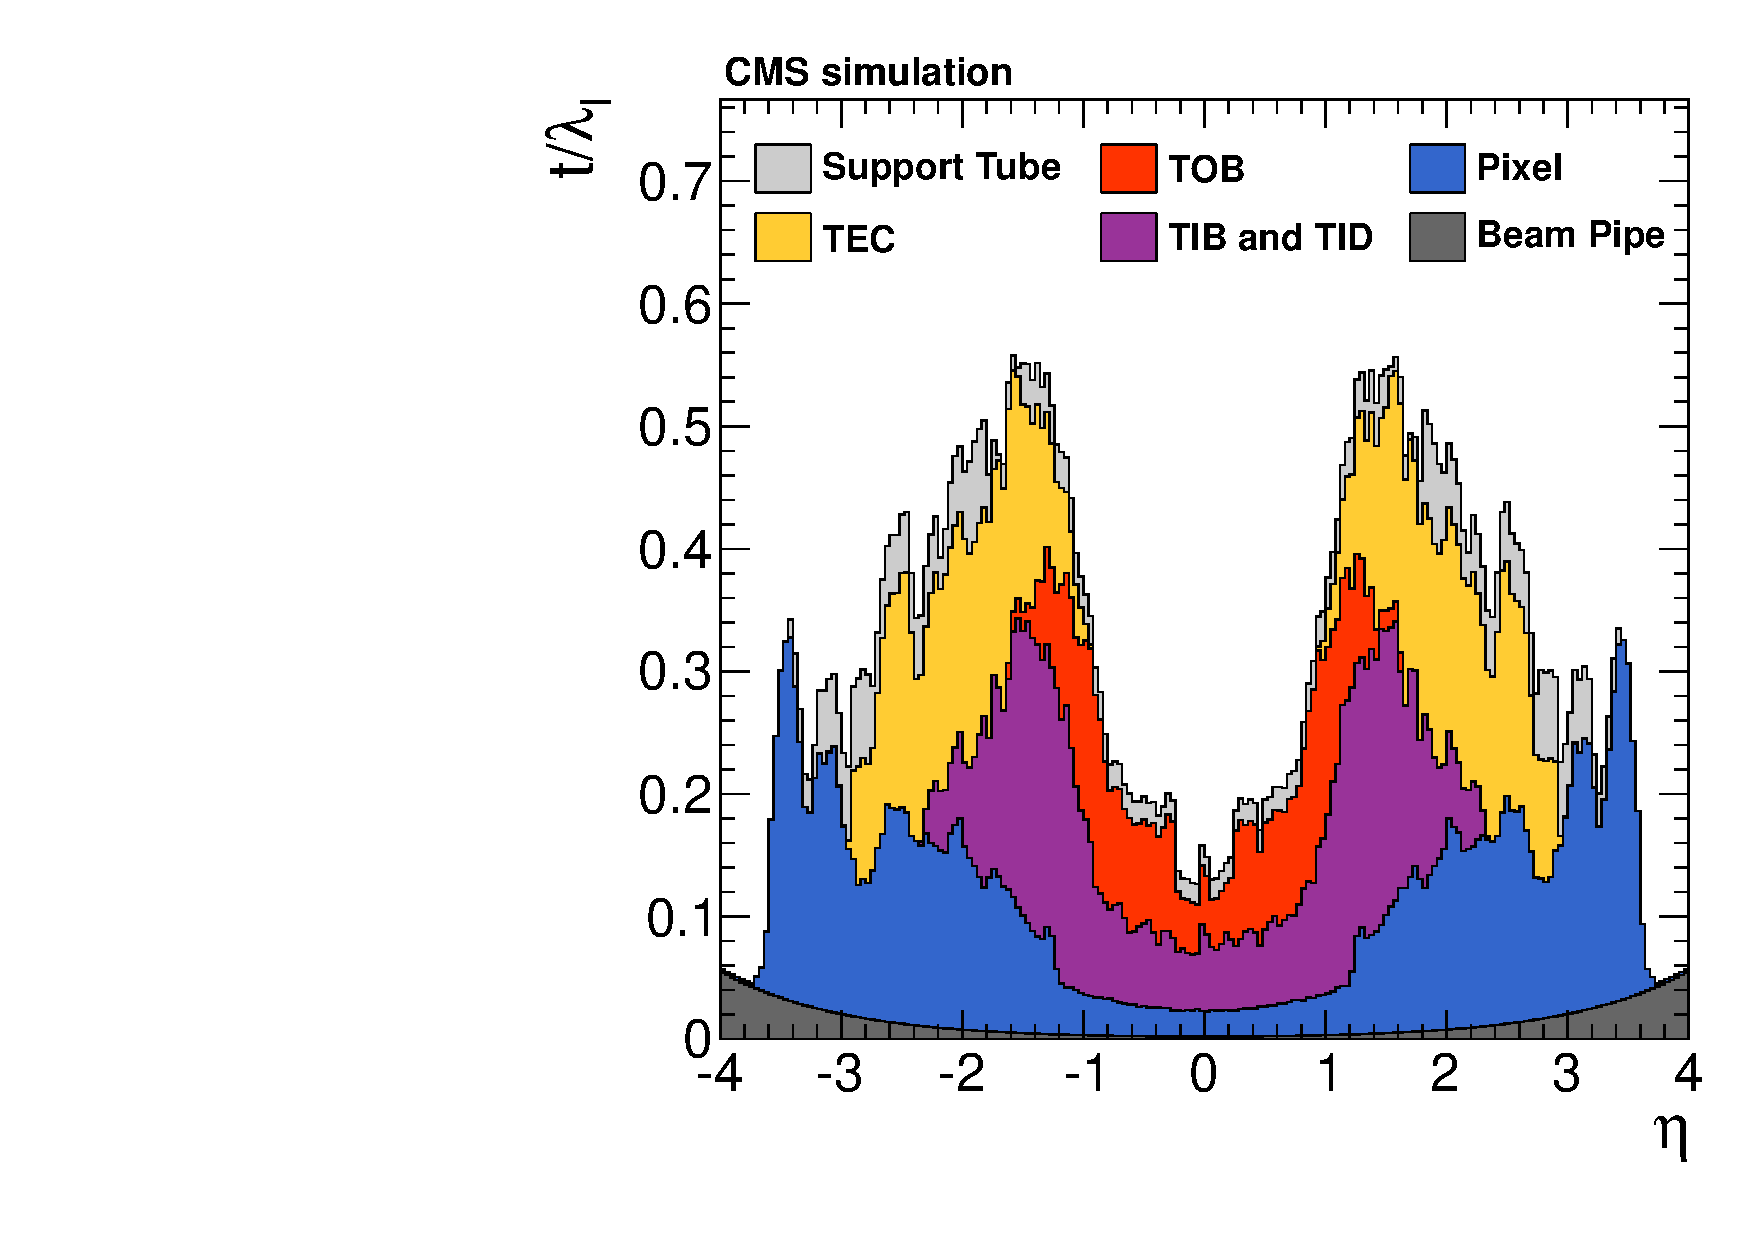
\includegraphics[width=0.4\textwidth]{cms_and_lhc/plots/cms_tracker_thickness_radiationL.pdf}
     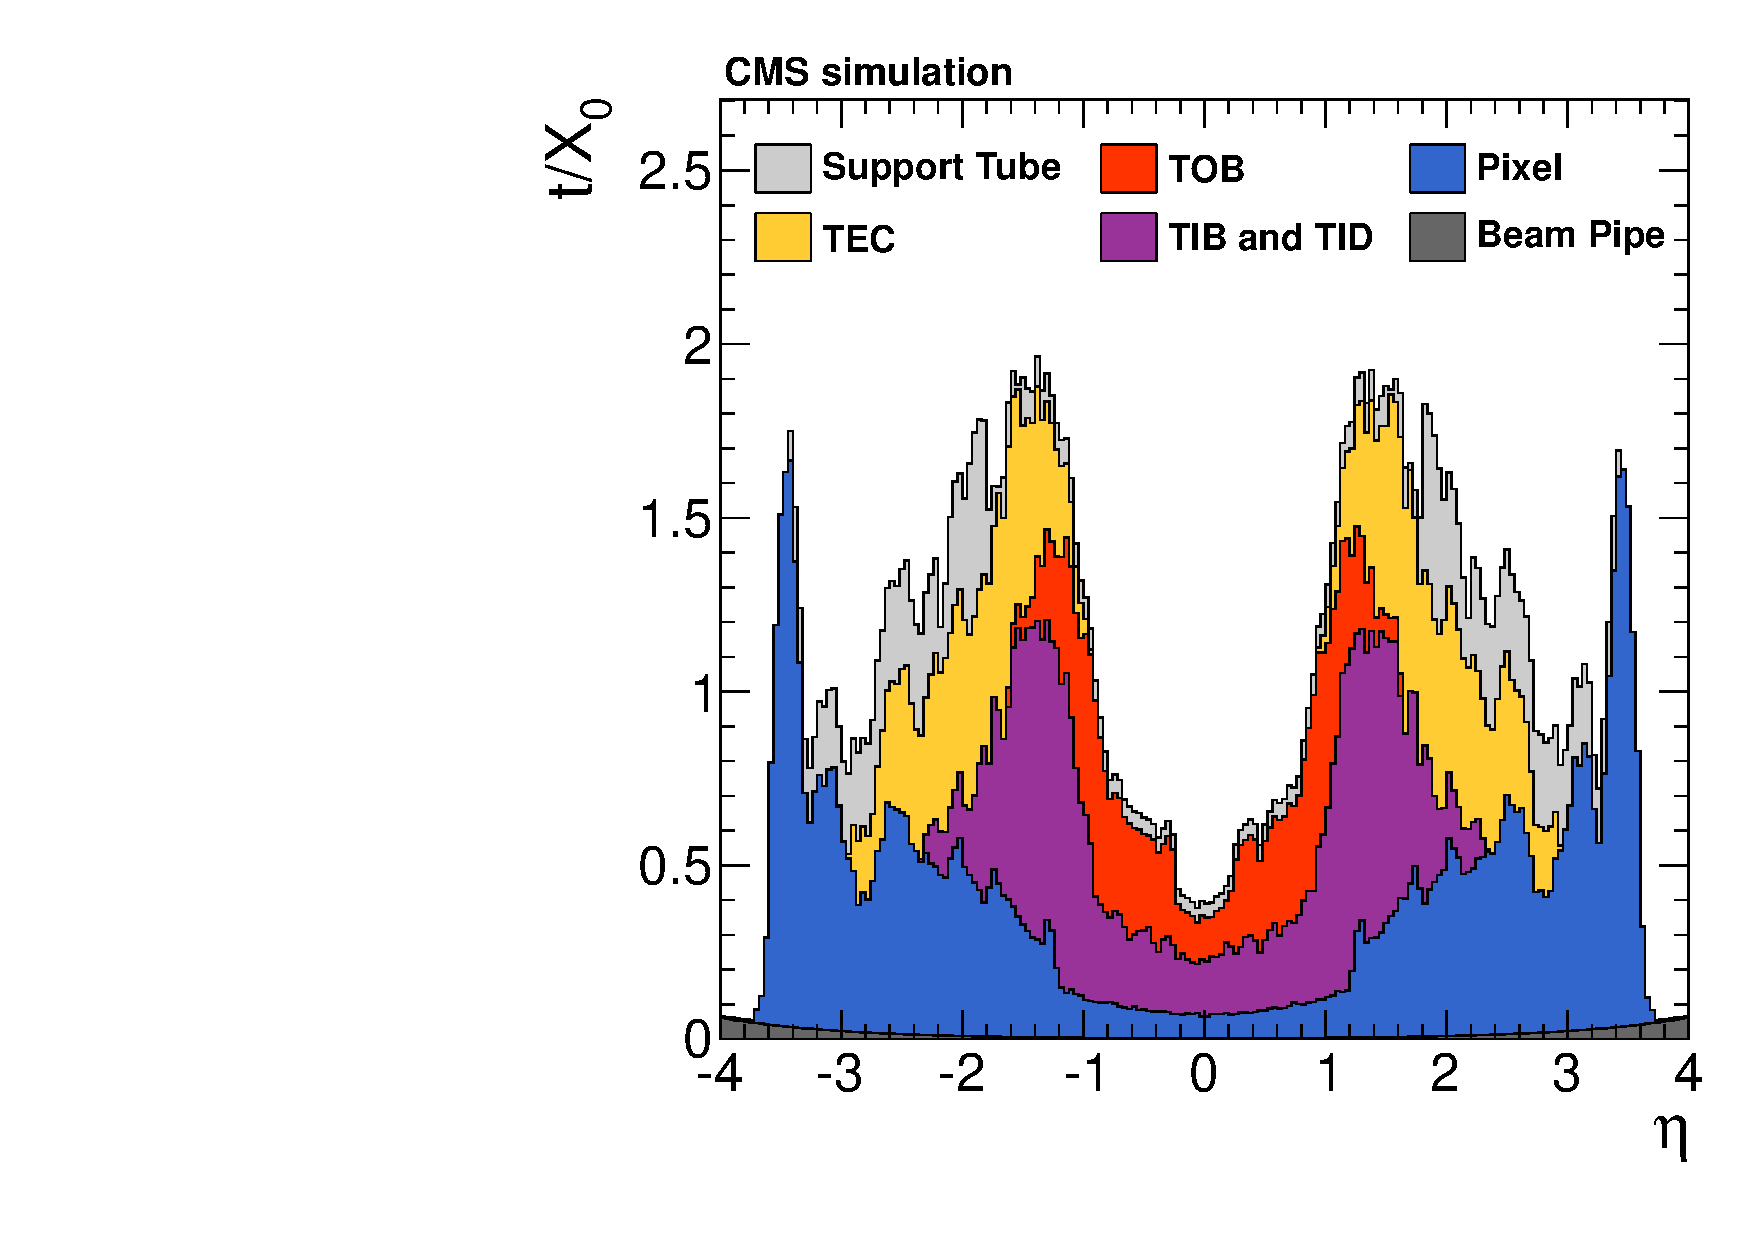
\includegraphics[width=0.4\textwidth]{cms_and_lhc/plots/cms_tracker_thickness_interactionL.pdf}
     \caption{
Total thickness $t$ of the inner tracker material expressed in units of interaction lengths 
$\lambda_{l}$ (left) and radiation lengths $X_{0}$ (right), as a function of the pseudorapidity $\eta$.
     }
     \label{fig:cms_tracker_thickness}
\end{figure*}



\subsection{Electromagnetic Calorimeter}
The electromagnetic calorimeter (ECAL) is a homogeneous calorimeter made of lead 
tungstate $(\textrm{PbWO}_{4})$ crystals. There are 61200 individual crystals mounted
in the barrel region with 360 crystals completing a ring in $\phi$ and 170 crystals
spanning the barrel $\eta$ range, $\abs\eta < 1.479$. The corresponding crystal
cross-section is approximately $0.0174 \times 0.0174$ in \etaphi, or about $22 \times 22 \textrm{mm}^{2}$
on the front face of a crystal. Twenty-two millimeters is also the Moli\`ere radius
for $(\textrm{PbWO}_{4})$, meaning, on average, an electromagnetic shower could be
contained by 4 crystals. The total crystal length of 230mm corresponds to a
radiation length of 25.8 $X_{0}$. 
As particles interact with the crystals, energy is deposited at a rate of about 4.5
photoelectrons per \MeV~\cite{dafinei_auffray_lecoq_schneegans_1994}.
To read-out the energy deposited in each barrel
crystal, there is an avalanch photodiode (APD) mounted to the backside-facing surface
of the crystal. For the endcap crystals, a more radiation hardened readout is used,
vacuum phototriodes (VPTs).






closed by 7324 crys- tals in each of the two endcaps. Vacuum phototriodes (VPTs) in the endcaps. The use of high density crystals has allowed the design of a calorimeter which is fast, has fine granularity and is radiation resistant, all important characteristics in the LHC environment. One of the driving criteria in the design was the capability to detect the decay to two photons of the postulated Higgs boson. This capability is enhanced by the good energy resolution provided by a homogeneous crystal calorimeter.

The electromagnetic calorimeter (ECAL) is a homogeneous calorimeter made of 61200 lead tungstate (PbWO4) crystals mounted in the central barrel part, closed by 7324 crys- tals in each of the two endcaps. A preshower detector is placed in front of the endcap crystals. Avalanche photodiodes (APDs) are used as photodetectors in the barrel and vacuum phototriodes (VPTs) in the endcaps. The use of high density crystals has allowed the design of a calorimeter which is fast, has fine granularity and is radiation resistant, all important characteristics in the LHC environment. One of the driving criteria in the design was the capability to detect the decay to two photons of the postulated Higgs boson. This capability is enhanced by the good energy resolution provided by a homogeneous crystal calorimeter.

at 18°C about 4.5 photoelectrons per MeV are collected in both APDs and VPTs.
The high density (8.28g/cm3), short radiation length (0.89cm) and small Molière radius (2.2 cm)

The scintillation decay time of these production crystals is of the same order of magnitude as the LHC bunch crossing time: about 80% of the light is emitted in 25 ns.

Barrel: 

hermetic homogeneous calorimeter made of lead tungstate (PbWO4) crystals. The barrel covers $\abs\eta < 1.479$ and the two endcap disks $1.479 < \abs\eta < 3.0$.
The barrel (endcap) crystal length of 23 (22) cm corresponds to 25.8 (24.7) radiation lengths, sufficient to contain more than 98\% of the energy of electrons and photons up to 1 TeV.
The crystal material also amounts to about one interaction length, causing about two thirds of the hadrons to start showering in the ECAL before entering the HCAL.
The crystal transverse size matches the small Moliere radius of PbWO4, 2.2cm. This fine transverse granularity makes it possible to fully resolve hadron and photon energy deposits as close as 5 cm from one another, for the benefit of exclusive particle identification in jets.
2.2 × 2.2 \cmsq, equivalent to 0.0174 × 0.0174 in the ($\eta$, $\phi$) plane.

Energy resolution:
\begin{equation}
\label{eqn:ecal_res}
\frac{\sigma}{E} = \frac{2.8\%}{\sqrt{E/\GeV}} \oplus \frac{12\%}{E/\GeV} \oplus 0.3\%
\end{equation}

typical ECAL electronics noise $\sigma ^{\text{ECAL}} _{\text{noise}}$ is measured to be $\approx$ 40 (150) \MeV per crystal in noise the barrel (endcaps).

\begin{figure*}[htbp]
\centering
     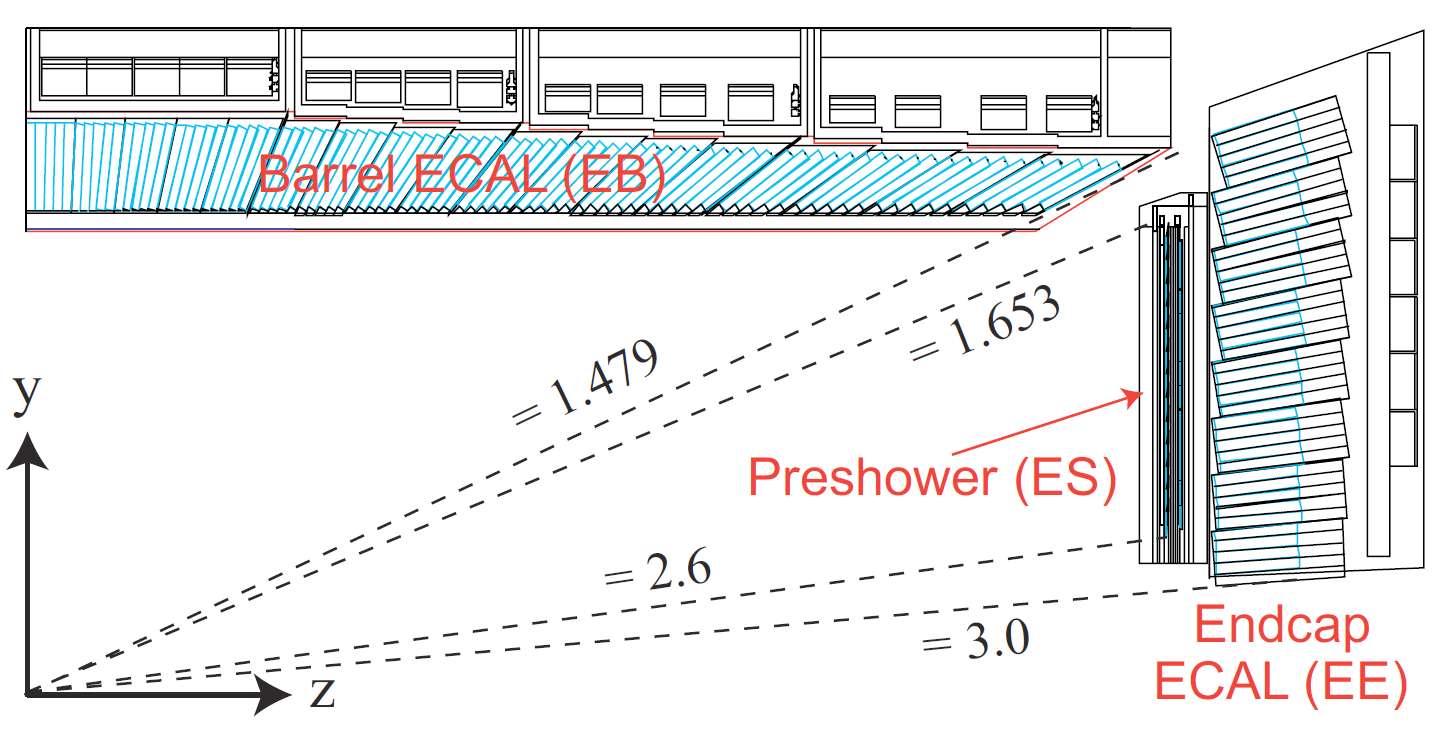
\includegraphics[width=0.8\textwidth]{cms_and_lhc/plots/cms_ecal.png}
     \caption{
     }
     \label{fig:cms_ecal}
\end{figure*}



\subsection{Hadronic Calorimeter}

The hadron calorimeters are particularly important for the measurement of hadron jets and neutrinos or exotic particles resulting in apparent missing transverse energy~\cite{CMS-Proposal}

radially restricted between the outer extent of the electromagnetic calorimeter (R = 1.77 m) and the inner extent of the magnet coil (R = 2.95 m).

Therefore, an outer hadron calorimeter or tail catcher is placed outside the solenoid complementing the barrel calorimeter. Beyond |η| = 3, the forward hadron calorimeters placed at 11.2 m from the interaction point extend the pseudorapidity coverage down to |η| = 5.2 using a Cherenkov-based, radiation-hard technology.

The HB is a sampling calorimeter covering the pseudorapidity range |η| < 1.3

flat brass absorber plates (table 5.1) aligned parallel to the beam axis

The plastic scintillator is divided into 16 η sectors, resulting in a segmentation (∆η,∆φ) = (0.087,0.087)

The total absorber thickness at 90◦ is 5.82 interaction lengths (λI ) HB effective thickness increases with polar angle (θ) as 1/sinθ, resulting in 10.6 λI at |η| = 1.3

Scintillator tile and wavelength shifting fibre concept to bring out the light. The CMS hadron calorimeter consists of about 70 000 tiles. plastic scintillator, chosen for its long-term stability and moderate radiation hardness.
 


HO
for |η| < 1.3
The total depth of the calorimeter system is thus extended to a minimum of 11.8 λI

HF
On average, 760 GeV per proton-proton interaction is deposited into the two forward calorimeters, compared to only 100 GeV for the rest of the detector.
Successful operation critically depends on the radiation hardness of the active material. This was the principal reason why quartz fibres (fused-silica core and polymer hard-cladding) were chosen as the active medium.
The calorimeter consists of a steel absorber structure that is composed of 5 mm thick grooved
plates. Fibres are inserted in these grooves.
full depth of the absorber (165 cm ≈ 10λI)
where Cherenkov radiation forms the basis of signal generation. Thus, the detector is essentially sensitive only to the electromag- netic shower core and is highly non-compensating (e/h ≈ 5).




hermetic sampling calorimeter consisting of several layers of brass absorber and plastic scintillator tiles. It surrounds the ECAL, with a barrel ($\abs\eta$ < 1.3) and two endcap disks ($1.3 < \abs\eta < 3.0$).
Almost six interaction lengths at normal incidence, and increases to over ten interaction lengths at larger pseudorapidities.
It is complemented by a tail catcher (HO), installed outside the solenoid coil. The HO material 
(1.4 interaction lengths at normal incidence) is used as an additional absorber. At small pseudorapidities ($\abs\eta < 0.25$), 
this thickness is enhanced to a total of three interaction lengths by a 20 cm-thick layer of steel. 
The total depth of the calorimeter system (including ECAL) is thus extended to a minimum of 
twelve interaction lengths in the barrel. In the endcaps, the thickness amounts to about ten interaction lengths.

individual towers with a cross section $\Delta\eta \times \Delta\phi = 0.087 \times 0.087$ for $\abs\eta < 1.6$ 
and $0.17 \times 0.17$ at larger pseudorapidities.

Energy resolution has been measured for the HB using test beams~\cite{Elvira:800406}, and is:
\begin{equation}
\label{eqn:hcal_res}
\frac{\sigma}{E} = \frac{115\%}{\sqrt{E/\GeV}} \oplus 5.5\%
\end{equation}
For HF hadronic energy resolution~\cite{Baiatian:951395},
\begin{equation}
\label{eqn:hcal_res}
\frac{\sigma}{E} = \frac{280\%}{\sqrt{E/\GeV}} \oplus 11\%
\end{equation}

typical HCAL electronics noise $\sigma ^{\text{HCAL}} _{\text{noise}}$ is measured to be $\approx$ 200 MeV per tower.

\begin{figure*}[htbp]
\centering
     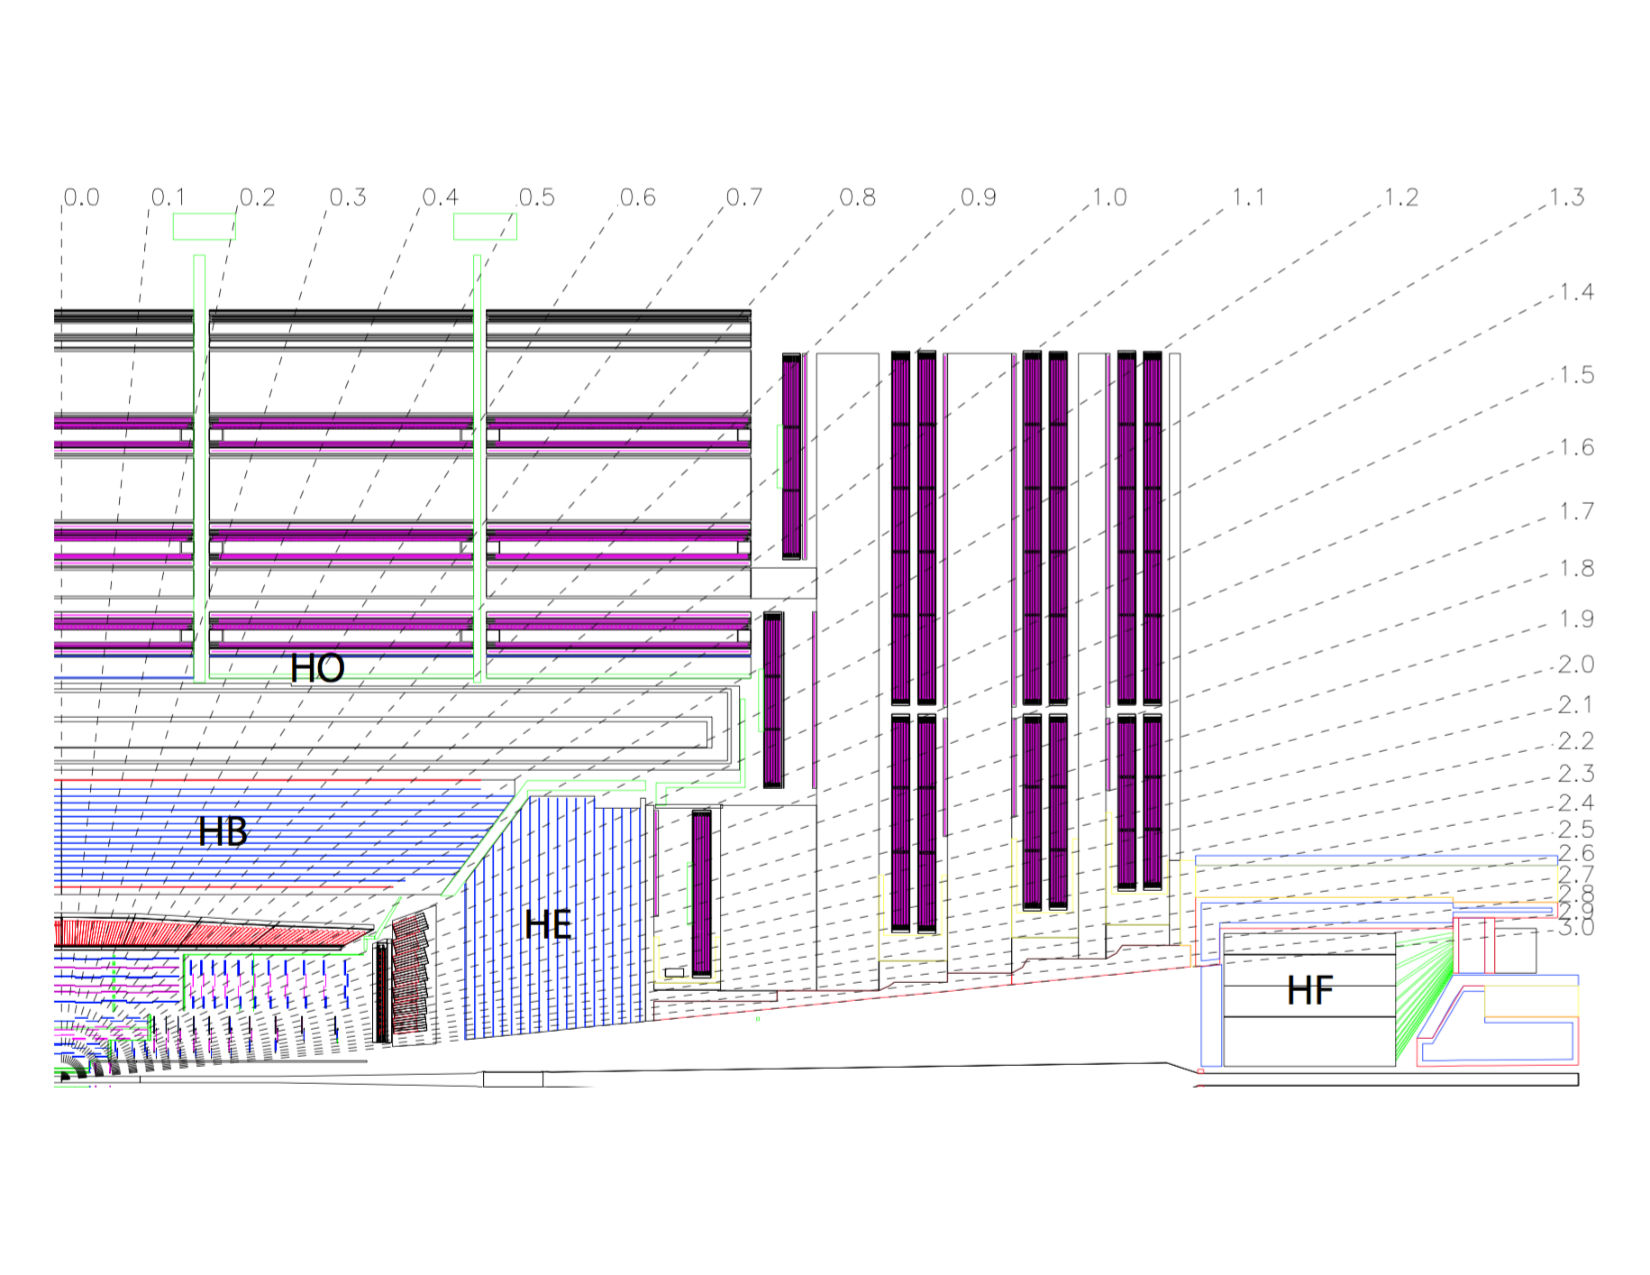
\includegraphics[width=0.8\textwidth]{cms_and_lhc/plots/cms_hcal.pdf}
     \caption{
Longitudinal view of the CMS detector showing the locations of the hadron barrel (HB), endcap (HE), outer (HO) and forward (HF) calorimeters.
     }
     \label{fig:cms_hcal}
\end{figure*}


\subsection{Muon System}

Muon system key to HZZ 4 muons.  Best momentum resolution over 4 electrons. Key to Higgs analysis.

The muon system has 3 functions: muon identification, momentum measurement, and triggering.

In the barrel region, where the neutron-induced background is small, the muon rate is low, and the 4-T magnetic field is uniform and mostly contained in the steel yoke, drift chambers with standard rectangular drift cells are used. The barrel drift tube (DT) chambers cover the pseudora- pidity region |η| < 1.2

In the 2 endcap regions of CMS, where the muon rates and background levels are high and the magnetic field is large and non-uniform, the muon system uses cathode strip chambers (CSC). With their fast response time, fine segmentation, and radiation resistance, the CSCs identify muons between |η| values of 0.9 and 2.4.

Because of the uncertainty in the eventual background rates and in the ability of the muon system to measure the correct beam-crossing time when the LHC reaches full luminosity, a com- plementary, dedicated trigger system consisting of resistive plate chambers (RPC) was added in both the barrel and endcap regions. The RPCs provide a fast, independent, and highly-segmented trigger with a sharp pT threshold over a large portion of the rapidity range (|η| < 1.6) of the muon system. The RPCs are double-gap chambers, operated in avalanche mode to ensure good operation at high rates. They produce a fast response, with good time resolution but coarser position reso- lution than the DTs or CSCs. They also help to resolve ambiguities in attempting to make tracks from multiple hits in a chamber.~\cite{1748-0221-8-03-T03001}.


\begin{figure*}[htbp]
\centering
     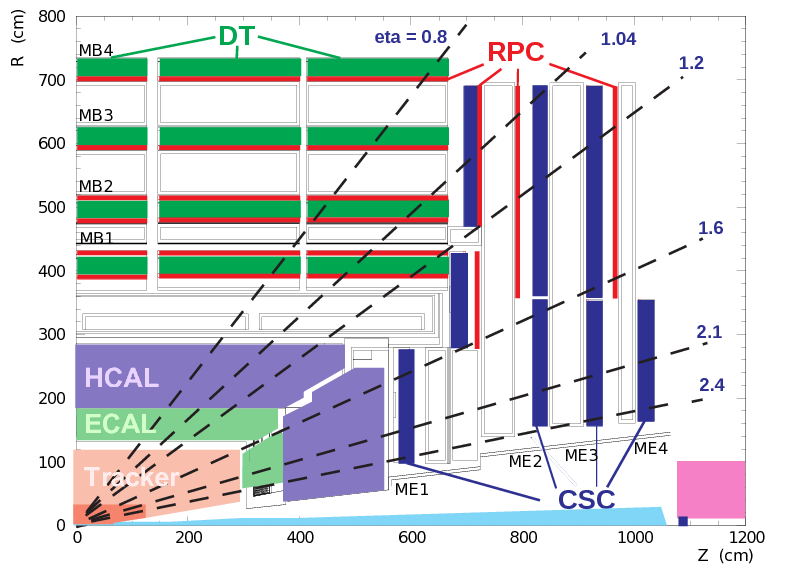
\includegraphics[width=1.0\textwidth]{cms_and_lhc/plots/cms_muon_syst.png}
     \caption{
Layout of one quadrant of CMS. The four DT stations in the barrel (MB1-MB4, green), the four CSC stations in the endcap (ME1-ME4, blue), and the RPC stations (red) are shown.
     }
     \label{fig:cms_muon_syst}
\end{figure*}



Outside the solenoid coil, the magnetic flux is returned through a yoke consisting of three 
layers of steel interleaved with four muon detector planes. Drift tube (DT) chambers and 
cathode strip chambers (CSC) detect muons in the regions $\abs\eta < 1.2$ and $0.9 < \abs\eta < 2.4$, 
respectively, and are complemented by a system of resistive plate chambers (RPC) covering the range $\abs\eta < 1.6$.

\subsubsection{Drift Tubes}
\subsubsection{Cathode Strip Chambers}
\subsubsection{Resistive Plate Chambers}
\subsection{Trigger and Data Acquisition}
40 MHz - high speed electronics capable of operating in close synchronization
trigger, L1, HLT
Significant upgrades of the L1 trigger during the first long shutdown of the LHC have benefitted this analysis, especially in the $\tauh\tauh$ channel. These upgrades improved the $\tauh$ identification at L1 by giving more flexibility to object isolation, allowing new techniques to suppress the contribution from additional $\Pp\Pp$ interactions per bunch
crossing, and to reconstruct the L1 $\tauh$ object in a fiducial region that matches more closely that of a true hadronic $\Pgt$ decay. The flexibility is achieved by employing high bandwidth optical links for data communication and large field-programmable gate arrays (FPGAs) for data processing.

\subsubsection{Level-1 Trigger}
\subsubsection{Aside for CaloL1 Duties and Online SW}
\subsubsection{HLT}
\subsubsection{Aside for 2018 Tau Trigger Updates}
\subsubsection{Aside for Phase-2 L1EG Discussion}
